Con questa nuova variante si propone una versione aggiornata di \textbf{\textit{All-in-One}}.\\
\\
In particolare si è deciso di agire sugli aspetti più deboli di \textit{All-in-One} e in generale del protocollo base GreenWUP.\\
Infatti con queste nuove modifiche è cambiato sia la semantica del tempo \textit{Jitter} di ogni \textit{receiver} sia la logica con cui viene impostato il numero di trasmissioni verso un nodo cached.

\subsection{Semantica del tempo Jitter}
Come succedeva per tutte le varianti proposte finora, compresa la versione base del protocollo, il tempo Jitter che ogni receiver aspetta prima di inviare il pacchetto CTS è calcolato in modo puramente aleatorio. Come già discusso questa soluzione non è delle migliori per cui si è deciso di attribuirgli una semantica più interessante.\\
In particolare ogni receiver calcola un tempo jitter considerando la quantità di energia utilizzabile. In questo modo il nodo sender riceverà molto probabilmente il primo pacchetto CTS non da un nodo qualunque ma dal nodo con più energia disponibile.\\
La nuova formula che definisce il tempo Jitter è quindi la seguente:
\[Jitter = \delta_{d} * (1-\delta_e) + \delta_r\]
con \(\delta_{d}\) che rappresenta il massimo delay consentito, \(\delta_{e}\) rappresenta la percentuale di energia attualmente disponibile normalizzata in \([0-1]\) e \(\delta_{r}\) che rappresenta, invece, un valore randomico.\\

\'E facile notare che adesso il valore finale di \textit{Jitter} dipende fortemente dal valore energetico che un nodo ha in un determinato istante. In particolare, minore è la percentuale di energia maggiore sarà il Jitter. La presenza di \(\delta_{r}\) è richiesta in quanto consente di evitare le collisioni nel momento in cui ci siano più nodi receiver con la stessa percentuale di energia.

\subsection{Decisione del numero di trasmissioni verso il nodo cached}
\'E stata inoltre modificata anche la logica con cui viene valorizzata la variabile \textit{txBeforeChangingRelayCached}.\\
Inizialmente, infatti, questa variabile, che regola in numero di trasmissioni verso il nodo cached (\textbf{riga 2, Codice \ref{code:checkForRelay}}), era stata impostata staticamente\footnote{Valore scelto ovviamente dopo una serie di tentativi, osservando i risultati ottenuti con vari valori.} a 3.\\
Grazie alle modifiche apportate ogni nodo è in grado di decidere ogni volta il numero di trasmissioni verso un determinato nodo cached basandosi su parametri che forniscono una valutazione del nodo cached. In questo modo è stato possibile aumentare il numero di utilizzi per quei nodi in grado di supportare l'incarico, mentre per altri nodi si è scelto un valore più basso in modo da evitare che questi esaurissero la propria energia.\\ 

Per fare ciò è stata necessaria la modifica al Jitter sopra descritta. Infatti, un nodo sender decide di impostare questo valore basandosi sul tempo che i vari receiver impiegano ad inviare il pacchetto CTS e, dato che questo dipende dalla loro energia residua, si può affermare che maggiore sarà l'energia del nodo receiver (di conseguenza minore sarà il Jitter calcolato) maggiore sarà anche il numero di trasmissioni che il nodo sender decide di fare verso il nodo cached in questione.\\

Nonostante il numero di trasmissioni sia variabile tra i vari nodi sender si è scelto comunque di fissare un tetto massimo, e ovviamente minimo, affinché non si concentri il traffico sempre verso gli stessi nodi.\\ Questo fenomeno potrebbe infatti risultare dannoso in scenari in cui c'è poco traffico e quindi si utilizzerebbero per tutto il lifetime della rete gli stessi next-hop.\\
In particolare il numero di ritrasmissioni che il sender sceglierà per un determinato nodo cache apparterrà all'intervallo \([1, 6]\).\\
Per la realizzazione di questa modifica sono, inoltre, state usate 3 nuovi variabili:

\begin{listing}[h]
    \caption{Nuove variabili usate per le modifiche}
    \label{code:variables_final2.0}
    \begin{minted}[mathescape, linenos, numbersep=10pt, gobble=0, fontsize=\small, frame=lines, framesep=2mm]{cpp}

double maxTxCache;
double minTxCache;
double factorTxCache = (minTxCache - maxTxCache) / 5;

    \end{minted}
\end{listing}\\

In particolare queste variabili aiutano a definire un mapping tra i tempi di attesa dei pacchetti CTS e l'intervallo \([1, 6]\) sopra citato:
\begin{itemize}
    \item \textit{maxTxCache} è un valore definito inizialmente da ogni nodo, calcolato usando la formula del Jitter ma considerando la massima energia. Questo valore corrisponde al migliore dei casi, ovvero, l'estremo superiore dell'intervallo, 6;
    \item \textit{minTxCache} è anch'esso calcolato inizialmente da tutti i nodi usando la formula del Jitter ma questa volta si considera solo il 50\% dell'energia disponibile. Questo corrisponde al caso "peggiore", infatti è associato all'estremo inferiore dell'intervallo, 1;
    \item \textit{factorTxCache} è invece un valore che permette di dividere l'intervallo\\ \([maxTxCache, minTxCache]\) nelle stesse parti dell'intervallo \([1, 6]\) in modo da avere un mapping corretto per ogni valore.
\end{itemize}

A questo punto, quando un nodo cached, durante la fase di Relay-Selection, riceve il pacchetto CTS da un vicino, dopo averlo memorizzato in cache, calcola anche il numero di trasmissioni da affidare a quest'ultimo usando la seguente funzione:

\begin{listing}[h]
    \caption{Funzione che restituisce il corretto numero di ritrasmissioni per un nodo cached}
    \label{code:getTxTimes_final2.0}
    \begin{minted}[mathescape, linenos, numbersep=10pt, gobble=0, fontsize=\small, frame=lines, framesep=2mm]{cpp}

int GreenWup::getTxTimes(double x) {
  if( x <= maxTxCache ) return 6;
  if( x >= minTxCache) return 1;

  int n = 7;
  double temp = maxTxCache;
  
  while(x > temp){
    temp += factorTxCache;
    n--;
  }
  return n;
}

    \end{minted}
\end{listing}\\

La funzione illustrata nel \textbf{Codice \ref{code:getTxTimes_final2.0}} prende in input un valore \textit{x} definito come il tempo trascorso tra l'invio del pacchetto RTS e la ricezione del pacchetto CTS\footnote{ovviamente eliminando tempi noti come quello necessario all'invio del CTS} e restituisce un intero \textit{n} appartenente all'intervallo \([1, 6]\), a seconda, ovviamente, della posizione di \textit{x} nell'intervallo \([maxTxCache, minTxCache]\).\\
\\

\newpage

Per completezza la \textbf{Figura \ref{fig:getTxTimes_final2.0}} mostra graficamente in che modo la funzione appena presentata restituisce un valore \textit{n} dato un valore in input \textit{x}.

\begin{figure}[h!]
  \begin{subfigure}[t]{0.9\linewidth}
    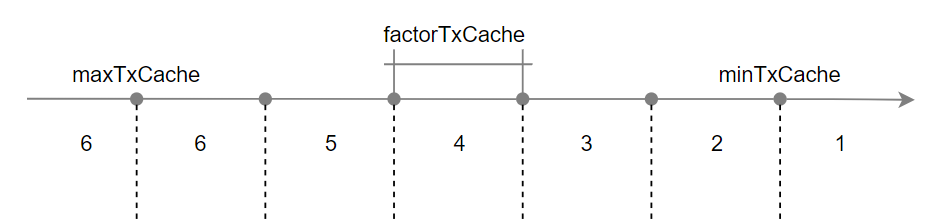
\includegraphics[width=1.1\linewidth]{Contents/Images/schemes/final2.0/getTxTrasmiss.PNG}
    \caption{TX Time for the WUR}
  \end{subfigure}
  \caption{Grafico dei valori di ritorno della funzione getTxTimes}
  \label{fig:getTxTimes_final2.0}
\end{figure}